\documentclass[letterpaper, 11pt]{memoir}

\usepackage[usenames,dvipsnames]{xcolor}
\usepackage{csquotes}
\usepackage[super]{nth}
\usepackage{enumitem}
  \setlist{itemsep=0mm}
\usepackage{graphbox}
\usepackage{sidecap} % Adds wide environment for full-width figures

%% Plots, figures and Tikz
\usepackage{tikz}
  \usetikzlibrary{arrows}
    \tikzset{>=stealth}
  \usetikzlibrary{backgrounds}
  \usetikzlibrary{chains}
  \usetikzlibrary{plotmarks}
  \usetikzlibrary{positioning}
  \usetikzlibrary{external}
    \tikzexternalize
    \tikzset{external/only named}
    \tikzset{external/mode=list and make}
    \tikzset{external/prefix=fig/}
    \tikzset{external/system call=%
        {lualatex \tikzexternalcheckshellescape -synctex=1 %
        -interaction=batchmode -jobname "\image" "\texsource"}%
    }
    \pgfkeys{/pgf/images/include external/.code={%
        \IfFileExists{#1.pdf}{%
          \includegraphics{{#1}.pdf}%
        }{%
          \includegraphics[draft]{{#1}.pdf}%
        }%
      }
    }
  \tikzset{
    blk/.style={
      rectangle, very thick, draw=red!50!black!50,
      top color=white, bottom color=red!50!black!20,
      font=\Large, minimum width=10mm, minimum height=8mm,
      anchor=west
    },
    tfblk/.append style={blk, font=\large, anchor=west},
    backblk/.style={
      very thick, top color=white, bottom color=blue!50!black!10
    },
    sum/.style={
      circle, very thick, draw=green!50!black!50,
      top color=white, bottom color=green!50!black!20,
      anchor=west
    },
    sum sign/.style={font=\tiny, inner sep=1.6pt},
    signal node/.style={circle, fill, inner sep=1pt},
    helper/.style={inner sep=0pt}
  }
\usepackage{pgfplots}
  \usepgfplotslibrary{groupplots}
  \usepgfplotslibrary{statistics}
  \pgfplotsset{compat=newest}
  \pgfplotsset{
    log ticks with fixed point,
    clip marker paths=true,
  }
\usepackage{pgfplotstable}
  \pgfplotstableset{
    every even row/.style={before row={\rowcolor[gray]{0.9}}},
    every head row/.style={before row=\toprule, after row=\midrule},
    every last row/.style={after row=\bottomrule},
  }
\usepackage{booktabs,colortbl}
\usepackage{tikz-timing}
\usepackage{circuitikz}
  \ctikzset{american voltages, inductor=cute}
\pgfdeclareshape{hcsr04}{
    \anchor{center}{\pgfpointorigin} % within the node, (0,0) is the center
    \anchor{text} % this is used to center the text in the node
    {\pgfpoint{-.5\wd\pgfnodeparttextbox}{-.5\ht\pgfnodeparttextbox}}
    
    % Pin Assignments
    \savedanchor\hcsrT{\pgfpoint{-1.2cm}{0.25cm}} % Pin Trig
    \anchor{Trig}{\hcsrT}
    \savedanchor\hcsrE{\pgfpoint{-1.2cm}{-0.25cm}} % Pin Echo
    \anchor{Echo}{\hcsrE}

    \savedanchor\hcsrG{\pgfpoint{0cm}{-1.5cm}} % Pin GND
    \anchor{GND}{\hcsrG}
    \savedanchor\hcsrV{\pgfpoint{0cm}{1.5cm}} % Pin 5V
    \anchor{Vcc}{\hcsrV}

    \foregroundpath{ % Border and Pin Names are drawn here    
        % Container
        \pgfsetlinewidth{0.5pt}
        \pgfpathrectanglecorners{\pgfpoint{1cm}{1.5cm}}{\pgfpoint{-1cm}{-1.5cm}}
        \pgfusepath{draw}
        
        % Pins
        \pgfsetlinewidth{0.9pt}
        \pgfpathmoveto{\pgfpoint{-1cm}{0.25cm}}
        \pgfpathlineto{\pgfpoint{-1.2cm}{0.25cm}}
        \pgfpathmoveto{\pgfpoint{-1cm}{-0.25cm}}
        \pgfpathlineto{\pgfpoint{-1.2cm}{-0.25cm}}
        \pgfusepath{draw}

        % Text
        \pgftext[bottom, right, at={\pgfpoint{-0.1cm}{1.6cm}}]{\normalsize HC-SR04}
        \pgftext[bottom, at={\pgfpoint{0cm}{-1.4cm}}]{\footnotesize GND}
        \pgftext[top, at={\pgfpoint{0cm}{1.4cm}}]{\footnotesize Vcc}
        \pgftext[left, at={\pgfpoint{-0.9cm}{0.25cm}}]{\footnotesize Trig}
        \pgftext[left, at={\pgfpoint{-0.9cm}{-0.25cm}}]{\footnotesize Echo}
    }
}
\pgfdeclareshape{arduino}{
    \anchor{center}{\pgfpointorigin} % within the node, (0,0) is the center
    \anchor{text} % this is used to center the text in the node
    {\pgfpoint{-.5\wd\pgfnodeparttextbox}{-.5\ht\pgfnodeparttextbox}}
    
    % Pin Assignments
    \savedanchor\arduinoa{\pgfpoint{-2.4cm}{-3.5cm}} % Pin A5
    \anchor{A5}{\arduinoa}
    \savedanchor\arduinob{\pgfpoint{-2.4cm}{-3cm}} % Pin A4
    \anchor{A4}{\arduinob}
    \savedanchor\arduinoc{\pgfpoint{-2.4cm}{-2.5cm}} % Pin A3
    \anchor{A3}{\arduinoc}
    \savedanchor\arduinod{\pgfpoint{-2.4cm}{-2cm}} % Pin A2
    \anchor{A2}{\arduinod}
    \savedanchor\arduinoe{\pgfpoint{-2.4cm}{-1.5cm}} % Pin A1
    \anchor{A1}{\arduinoe}
    \savedanchor\arduinof{\pgfpoint{-2.4cm}{-1cm}} % Pin A0
    \anchor{A0}{\arduinof}
    
    \savedanchor\arduinog{\pgfpoint{2.4cm}{-3.5cm}} % Pin D0
    \anchor{D0}{\arduinog}
    \savedanchor\arduinoh{\pgfpoint{2.4cm}{-3cm}} % Pin D1
    \anchor{D1}{\arduinoh}
    \savedanchor\arduinoi{\pgfpoint{2.4cm}{-2.5cm}} % Pin D2
    \anchor{D2}{\arduinoi}
    \savedanchor\arduinoj{\pgfpoint{2.4cm}{-2cm}} % Pin D3
    \anchor{D3}{\arduinoj}
    \savedanchor\arduinok{\pgfpoint{2.4cm}{-1.5cm}} % Pin D4
    \anchor{D4}{\arduinok}
    \savedanchor\arduinol{\pgfpoint{2.4cm}{-1cm}} % Pin D5
    \anchor{D5}{\arduinol}
    \savedanchor\arduinom{\pgfpoint{2.4cm}{-0.5cm}} % Pin D6
    \anchor{D6}{\arduinom}
    \savedanchor\arduinon{\pgfpoint{2.4cm}{0cm}} % Pin D7
    \anchor{D7}{\arduinon}
    \savedanchor\arduinoo{\pgfpoint{2.4cm}{0.5cm}} % Pin D8
    \anchor{D8}{\arduinoo}
    \savedanchor\arduinop{\pgfpoint{2.4cm}{1cm}} % Pin D9
    \anchor{D9}{\arduinop}
    \savedanchor\arduinoq{\pgfpoint{2.4cm}{1.5cm}} % Pin D10
    \anchor{D10}{\arduinoq}
    \savedanchor\arduinor{\pgfpoint{2.4cm}{2cm}} % Pin D11
    \anchor{D11}{\arduinor}
    \savedanchor\arduinos{\pgfpoint{2.4cm}{2.5cm}} % Pin D12
    \anchor{D12}{\arduinos}
    \savedanchor\arduinot{\pgfpoint{2.4cm}{3cm}} % Pin D13
    \anchor{D13}{\arduinot}
    
    \savedanchor\arduinou{\pgfpoint{-2.4cm}{2.5cm}} % Pin AREF
    \anchor{AREF}{\arduinou}
    \savedanchor\arduinov{\pgfpoint{-2.4cm}{3cm}} % Pin RST
    \anchor{RST}{\arduinov}
    
    \savedanchor\arduinow{\pgfpoint{0.1cm}{-4.4cm}} % Pin GND
    \anchor{GND}{\arduinow}
    \savedanchor\arduinox{\pgfpoint{-1cm}{4.4cm}} % Pin 3V
    \anchor{3V}{\arduinox}
    \savedanchor\arduinoy{\pgfpoint{-0.5cm}{4.4cm}} % Pin 5V
    \anchor{5V}{\arduinoy}
    \savedanchor\arduinoz{\pgfpoint{1cm}{4.4cm}} % Pin Vin
    \anchor{VIN}{\arduinoz}
    
    \foregroundpath{ % Border and Pin Names are drawn here
    
        % Container
        \pgfsetlinewidth{0.5pt}
        \pgfpathrectanglecorners{\pgfpoint{2cm}{4cm}}{\pgfpoint{-2cm}{-4cm}}
        \pgfusepath{draw}
        
        % Analog Input Pins
        \pgfsetlinewidth{0.9pt}
        \pgfpathmoveto{\pgfpoint{-2cm}{-3.5cm}}
        \pgfpathlineto{\pgfpoint{-2.4cm}{-3.5cm}}
        \pgfpathmoveto{\pgfpoint{-2cm}{-3cm}}
        \pgfpathlineto{\pgfpoint{-2.4cm}{-3cm}}
        \pgfpathmoveto{\pgfpoint{-2cm}{-2.5cm}}
        \pgfpathlineto{\pgfpoint{-2.4cm}{-2.5cm}}
        \pgfpathmoveto{\pgfpoint{-2cm}{-2cm}}
        \pgfpathlineto{\pgfpoint{-2.4cm}{-2cm}}
        \pgfpathmoveto{\pgfpoint{-2cm}{-1.5cm}}
        \pgfpathlineto{\pgfpoint{-2.4cm}{-1.5cm}}
        \pgfpathmoveto{\pgfpoint{-2cm}{-1cm}}
        \pgfpathlineto{\pgfpoint{-2.4cm}{-1cm}}
        \pgfusepath{draw}
        
        % Digital Input/Output Pins
        \pgfpathmoveto{\pgfpoint{2cm}{-3.5cm}}
        \pgfpathlineto{\pgfpoint{2.4cm}{-3.5cm}}
        \pgfpathmoveto{\pgfpoint{2cm}{-3cm}}
        \pgfpathlineto{\pgfpoint{2.4cm}{-3cm}}
        \pgfpathmoveto{\pgfpoint{2cm}{-2.5cm}}
        \pgfpathlineto{\pgfpoint{2.4cm}{-2.5cm}}
        \pgfpathmoveto{\pgfpoint{2cm}{-2cm}}
        \pgfpathlineto{\pgfpoint{2.4cm}{-2cm}}
        \pgfpathmoveto{\pgfpoint{2cm}{-1.5cm}}
        \pgfpathlineto{\pgfpoint{2.4cm}{-1.5cm}}
        \pgfpathmoveto{\pgfpoint{2cm}{-1cm}}
        \pgfpathlineto{\pgfpoint{2.4cm}{-1cm}}
        \pgfpathmoveto{\pgfpoint{2cm}{-0.5cm}}
        \pgfpathlineto{\pgfpoint{2.4cm}{-0.5cm}}
        \pgfpathmoveto{\pgfpoint{2cm}{0cm}}
        \pgfpathlineto{\pgfpoint{2.4cm}{0cm}}
        \pgfpathmoveto{\pgfpoint{2cm}{0.5cm}}
        \pgfpathlineto{\pgfpoint{2.4cm}{0.5cm}}
        \pgfpathmoveto{\pgfpoint{2cm}{1cm}}
        \pgfpathlineto{\pgfpoint{2.4cm}{1cm}}
        \pgfpathmoveto{\pgfpoint{2cm}{1.5cm}}
        \pgfpathlineto{\pgfpoint{2.4cm}{1.5cm}}
        \pgfpathmoveto{\pgfpoint{2cm}{2cm}}
        \pgfpathlineto{\pgfpoint{2.4cm}{2cm}}
        \pgfpathmoveto{\pgfpoint{2cm}{2.5cm}}
        \pgfpathlineto{\pgfpoint{2.4cm}{2.5cm}}
        \pgfpathmoveto{\pgfpoint{2cm}{3cm}}
        \pgfpathlineto{\pgfpoint{2.4cm}{3cm}}
        \pgfusepath{draw}
        
        % AREF, RST Pins
        \pgfpathmoveto{\pgfpoint{-2cm}{2.5cm}}
        \pgfpathlineto{\pgfpoint{-2.4cm}{2.5cm}}
        \pgfpathmoveto{\pgfpoint{-2cm}{3cm}}
        \pgfpathlineto{\pgfpoint{-2.4cm}{3cm}}
        \pgfusepath{draw}
        
        % GND Pin
        \pgfpathmoveto{\pgfpoint{0.1cm}{-4cm}}
        \pgfpathlineto{\pgfpoint{0.1cm}{-4.4cm}}
        \pgfusepath{draw}
        
        % Power Pins
        \pgfpathmoveto{\pgfpoint{-1cm}{4cm}}
        \pgfpathlineto{\pgfpoint{-1cm}{4.4cm}}
        \pgfpathmoveto{\pgfpoint{-0.5cm}{4cm}}
        \pgfpathlineto{\pgfpoint{-0.5cm}{4.4cm}}
        \pgfpathmoveto{\pgfpoint{1cm}{4cm}}
        \pgfpathlineto{\pgfpoint{1cm}{4.4cm}}
        \pgfusepath{draw}

        % Arduino UNO Board Name
        \pgftext[bottom,at={\pgfpoint{0cm}{1.6cm}}]{\normalsize Arduino}
        %\pgftext[bottom,at={\pgfpoint{-0.25cm}{1.15cm}}]{\normalsize UNO}
        
        % Analog Input Pin Names
        \pgftext[bottom,rotate=-90,at={\pgfpoint{2.3cm}{-1.3cm}}]{\footnotesize Analog Input}
        \pgftext[center,at={\pgfpoint{-1.6cm}{-3.5cm}}]{\footnotesize A5}
        \pgftext[center,at={\pgfpoint{-1.6cm}{-3cm}}]{\footnotesize A4}
        \pgftext[center,at={\pgfpoint{-1.6cm}{-2.5cm}}]{\footnotesize A3}
        \pgftext[center,at={\pgfpoint{-1.6cm}{-2cm}}]{\footnotesize A2}
        \pgftext[center,at={\pgfpoint{-1.6cm}{-1.5cm}}]{\footnotesize A1}
        \pgftext[center,at={\pgfpoint{-1.6cm}{-1cm}}]{\footnotesize A0}
        
        % Digital Input/Output Pin Names
        \pgftext[bottom,rotate=90,at={\pgfpoint{-0.3cm}{-1.3cm}}]{\footnotesize Digital Input/Output}
        \pgftext[center,at={\pgfpoint{1.6cm}{-3.5cm}}]{\footnotesize D0}
        \pgftext[center,at={\pgfpoint{1.6cm}{-3cm}}]{\footnotesize D1}
        \pgftext[center,at={\pgfpoint{1.6cm}{-2.5cm}}]{\footnotesize D2}
        \pgftext[center,at={\pgfpoint{1.6cm}{-2cm}}]{\footnotesize D3}
        \pgftext[center,at={\pgfpoint{1.6cm}{-1.5cm}}]{\footnotesize D4}
        \pgftext[center,at={\pgfpoint{1.6cm}{-1cm}}]{\footnotesize D5}
        \pgftext[center,at={\pgfpoint{1.6cm}{-0.5cm}}]{\footnotesize D6}
        \pgftext[center,at={\pgfpoint{1.6cm}{0cm}}]{\footnotesize D7}
        \pgftext[center,at={\pgfpoint{1.6cm}{0.5cm}}]{\footnotesize D8}
        \pgftext[center,at={\pgfpoint{1.6cm}{1cm}}]{\footnotesize D9}
        \pgftext[center,at={\pgfpoint{1.6cm}{1.5cm}}]{\footnotesize D10}
        \pgftext[center,at={\pgfpoint{1.6cm}{2cm}}]{\footnotesize D11}
        \pgftext[center,at={\pgfpoint{1.6cm}{2.5cm}}]{\footnotesize D12}
        \pgftext[center,at={\pgfpoint{1.6cm}{3cm}}]{\footnotesize D13}
        
        % RST, AREF Pin Names
        \pgftext[center,at={\pgfpoint{-1.5cm}{2.5cm}}]{\footnotesize AREF}
        \pgftext[center,at={\pgfpoint{-1.6cm}{3cm}}]{\footnotesize RST}
        
        % GND Pin Name
        \pgftext[top,at={\pgfpoint{0.1cm}{-3.6cm}}]{\footnotesize GND}
        
        % Power Pin Names
        \pgftext[top,at={\pgfpoint{0.1cm}{3.5cm}}]{\small Power}
        \pgftext[top,at={\pgfpoint{-1cm}{3.8cm}}]{\footnotesize 3V}
        \pgftext[top,at={\pgfpoint{-0.5cm}{3.8cm}}]{\footnotesize 5V}
        \pgftext[top,at={\pgfpoint{1cm}{3.8cm}}]{\footnotesize Vin}
        
    }
}

\usepackage{minted}
  \definecolor{codebg}{gray}{0.97}
  \newminted[inocode]{arduino}{
    autogobble
  }
  \newmintinline[inocodei]{arduino}{bgcolor=codebg}
  %\newmintedfile[inofile]{arduino}{linenos}
\usepackage{mdframed}
  \surroundwithmdframed[backgroundcolor=codebg]{inocode}
  \newcommand{\inofile}{\begingroup
    \catcode`_=12 \doinofile}
  \newcommand{\doinofile}[1]{%
    \begin{mdframed}[
        backgroundcolor=codebg,
        frametitle={\space#1\space},
        frametitleaboveskip=-\ht\strutbox,
        frametitlealignment=\raggedleft
      ]
      \inputminted[linenos, fontsize=\small]{arduino}{code/#1}      
    \end{mdframed}
    \endgroup
  }

\usepackage{accsupp} % Fix for not copying line numbers in minted
  \newcommand\emptyaccsupp[1]{\BeginAccSupp{ActualText={}}#1\EndAccSupp{}}
  \let\theHFancyVerbLine\theFancyVerbLine
  \def\theFancyVerbLine{\rmfamily\tiny\emptyaccsupp{\arabic{FancyVerbLine}}}

\usepackage{siunitx}
  \sisetup{locale=US}
\usepackage[style=numeric-comp, sorting=none,
            useprefix=true, uniquename=false, uniquelist=false,
            maxnames=2, maxbibnames=8, backend=biber]{biblatex}
  \renewbibmacro{in:}{%
    \ifentrytype{article}{}{\printtext{\bibstring{in}\intitlepunct}}%
  }
  \addbibresource{bib.bib}

\usepackage{etoolbox}
\usepackage[hidelinks, pdfusetitle]{hyperref}

%% Control float placement
\renewcommand{\topfraction}{0.9}	% max fraction of floats at top
\renewcommand{\bottomfraction}{0.9}	% max fraction of floats at bottom
\setcounter{topnumber}{2}
\setcounter{bottomnumber}{2}
\setcounter{totalnumber}{4}


%% Document markup
\newcommand{\pending}[1]{\textbf{\emph{Pending:} #1}} % Stuff that needs done

\begin{document}

%! TeX root = main.tex

%% Title page, based on \titleTH in https://www.ctan.org/pkg/titlepages
\begin{titlingpage}
  \begingroup
  \raggedleft
  \vspace*{\baselineskip}
  {\Large Dimas Abreu Archanjo Dutra}\\[0.167\textheight]
  {\bfseries ~}\\[\baselineskip]
  {\textcolor{Blue}{\Huge Embedded System Programming with Arduino and C++}}\\[\baselineskip]
  {\small ~}\par
  \vfill
%  {Based on \emph{Embedded Controllers Using C and Arduino/2E}, by James M. Fiore
%    \\ 
\includegraphics{img/cc-by-nc-sa.pdf}}\par
%  \vspace*{3\baselineskip}
  \endgroup
\end{titlingpage}

%%% Local Variables:
%%% TeX-master: "main"
%%% eval: (adaptive-wrap-prefix-mode t)
%%% eval: (visual-line-mode t)
%%% eval: (nlinum-mode t)
%%% TeX-engine: luatex
%%% End:

\chapter{Introduction}
Embedded systems \parencite{leveson_embedded_2003} are special-purpose computer systems---composed of a processor, memory, software, and peripherals for input and ouput---that are embedded into a larger mechanical or electronic system.
Embedded systems are different from general-purpose computers such as desktops, laptops, mobile phones, and tablets because they typically run a single program which is tightly integrated to the accompanying hardware it is embedded within.
Their function is often to control or monitor a machine, which requires their program to react in real-time to sensor information or user input.

Arduino is a popular starting point for learning embedded systems today.
According to its \href{https://www.arduino.cc/en/Guide/Introduction}{official website}, 
``Arduino is an open-source electronics platform based on easy-to-use hardware and software'' \parencite{arduino_what_2018}.
It comprises of three main elements: 
hardware boards, the most famous of which is the Arduino Uno, shown in Fig.~\ref{fig:arduino_uno};
a microcontroller programming interface (API) and libraries in the C++ programming language, known as the \emph{Arduino language};
and an integrated development environment, the Arduino IDE.
Its low price, usability, and extensive community support make it an excelent entry point for learning embedded systems and a rapid prototyping tool for experts.

\begin{figure}[t]
  %\begin{wide}
    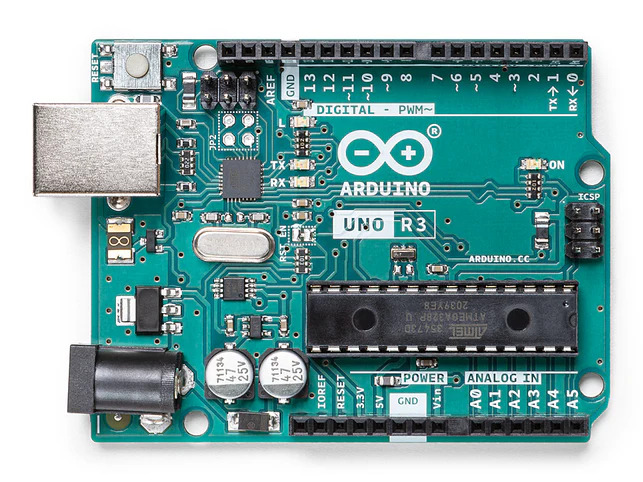
\includegraphics[width=0.5\textwidth]{img/arduino_uno_rev3}%
    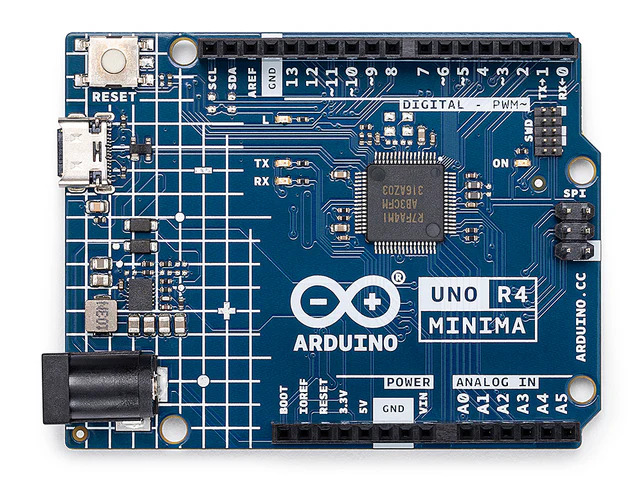
\includegraphics[width=0.5\textwidth]{img/arduino_uno_rev4}%
    \\ \scriptsize
    Source: \url{https://store.arduino.cc/collections/edu-boards}, under the \href{https://creativecommons.org/licenses/by-sa/3.0/legalcode}{Creative Commons Attribution ShareAlike 3.0} license.
    \caption{Arduino Uno Board Revisions Rev3 (R3) and R4 Minima.}
    \label{fig:arduino_uno}
  %\end{wide}
\end{figure}

This book is a introduction to embedded system programming with Arduino and C++.
Its main goal is laying out the foundations to understand the basic syntax of C++ and the while highlighting the unique aspects that distinguish embedded systems programming.
Its goal is enable readers to embed Arduinos or similar boards in their projects, leveraging existing libraries and frameworks instead of writing everything from scratch.
By understanding the core principles, readers will be able to integrate third-party code, modify existing solutions to fit their needs, build upon open-source projects, and even use AI in the software development process.
This approach also fosters good software engineering practices, such as code reuse, modular design, and systematic testing for robustness and correctness


\section{Platforms}
A defining characteristic of embedded systems is that the software is tightly coupled to the hardware it runs on.
Because of this, it is crucial to test your code on a physical hardware board to ensure proper functionality. Fortunately, many embedded platforms are affordable and widely available, making it easy to acquire a board for hands-on development.

Recommended boards for this book are:
\begin{description}
\item[Arduino Uno Rev3]
  The classic entry-level embedded platform, with many tutorials, example projects, libraries, drivers, and compatible hardware that snap in as Arduino Shields to extend its capabilities.
  The official, Arduino-branded device costs \SI{27}[\$]{} but, as its hardware design is open, fully compatible clones can be found for as low as \SI{8}[\$]{}.
  With only \SI{2}{KB} of RAM, it is resouce-constrained yet can still drive truly impressive projects.
  It is also a very forgiving board, robust against short-circuiting its pins, slight overvoltage, and general mishandling.
\item[Arduino UNO R4]
  A cheaper (\SI{20}[\$]{}) and more capable version of the Rev3, the UNO R4 has better performance and more features while maintaining the same form factor and voltage levels.
  It offers improved processing power, more memory, and additional peripherals, making it suitable for a broader range of projects.
  An excellent choice if you need more capability than the Rev3 but still prefer to stick with the familiar Arduino environment.
  A wireless version with Wi-Fi and bluetooth is also available for \SI{27.50}[\$]{}.
\item[ESP32]
  A family of low-cost platforms, starting at below \SI{5}[\$]{}, that offer a lot of performance.
  All boards feature built-in wireless communication (Wi-Fi and Bluetooth) and dual-core processors.
  The ESP32 is a great choice for projects involving connectivity or real-time processing.
  It can be programmed in C/C++, Python, Lua, and other languages.
\item[Raspberry Pi Pico 2]
  A highly capable option, starting at around \SI{5}[\$]{}, with dual-core ARM architecture and ample memory.
  Offers wireless capabilities in some variants and is compatible with both C++ and MicroPython, making it suitable for a variety of coding environments.
  The Raspberry Pi Pico is particularly beneficial for users who want a small, affordable board with substantial memory and processing power.
\end{description}

Simulation can also be a valuable tool, especially in the early stages of development or when hardware is not immediately accessible.
Simulators allow you to prototype, debug, and test code without the need for physical deployment, though they may not always capture the full range of hardware interactions.
They are also often used in automated testing and continuous integration (CI), allowing developers to catch and fix bugs early.

Recommended simulation environments for this book are:
\begin{description}
\item[Wokwi] 
  An extensible online digital electronics simulator that runs for free on a web browser.
  Wokwi can simulate Arduino, ESP32, STM32, and Raspberry Pi Pico.
  It can simulate multiple external hardware boards and the simulated IoT devices can connect to the internet.
  The supported programming languages include C/C++, Python, and Rust.
  Wokwi does not support analog simulation, however.\\
  \url{https://wokwi.com}
\item[TinkerCad Circuits] 
  A simple, introductory Arduino simulator that has some analog simulation capabilities.
  It runs on a web browser and has some external hardware boards implemented.\\
  \url{https://www.tinkercad.com/circuits}
\end{description}

Most examples in this book can be done either in a hardware board or in simulation.
For best learning, however, familiarity with hardware is important.
Having a physical board on hand is also essential for using what you learn in personal, academic, and professional projects, beyond the book examples, which is the ultimate goal of the book.

\section{Hello World on the Wokwi Simulator}

Hello World is the first program we will see on the Arduino to introduce the structure of the code and how to send information from the Arduino to a development computer.
The program is shown in Fig.~\ref{fig:wokwi-hello}, which also has a \href{https://wokwi.com/projects/420387835399008257}{link for opening it on the Wokwi simulator}.

\begin{figure}[b]
  \begin{wide}
    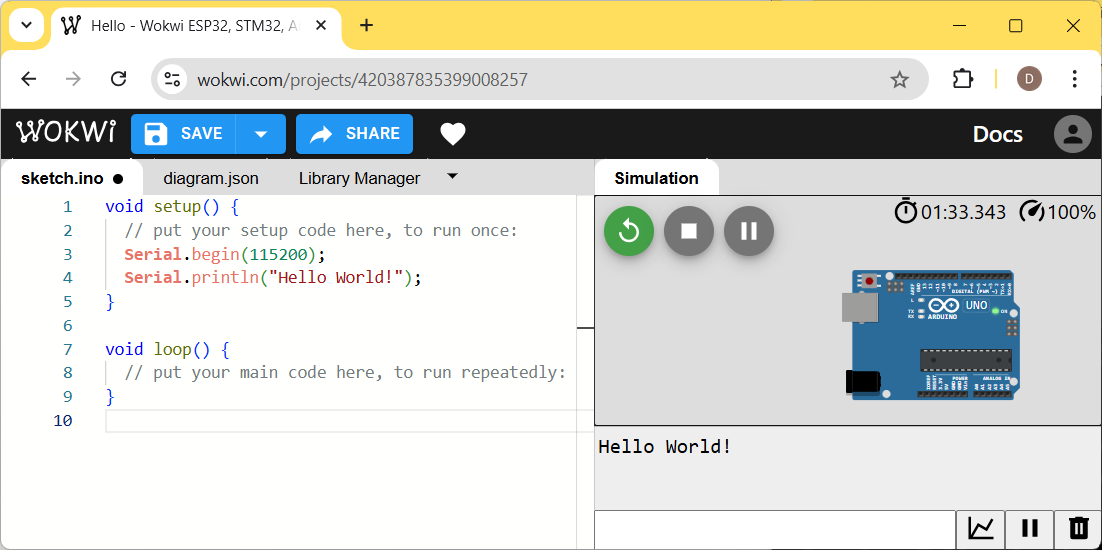
\includegraphics[width=\textwidth]{img/wokwi-hello.png}
    \\ \scriptsize
    Access this on \url{https://wokwi.com/projects/420387835399008257}
    \caption{Hello World program on the Wokwi simulator.}
    \label{fig:wokwi-hello}
  \end{wide}
\end{figure}

The program has two main blocks: the \texttt{setup} and \texttt{loop} functions.
Each function consists of the statements, or lines of code, between the curly braces \texttt{\{\}} that follow the function name.
In the code of Fig.~\ref{fig:wokwi-hello}, the \texttt{setup} function is in lines 1--5 and the \texttt{loop} function, between lines 7--9, is empty.
All the text after the characters \texttt{//}, which is typeset in grey, are comments and have no effect in the program's logic.

The Arduino program starts by executing the \texttt{setup} function which, as the name implies, usually initializes the device.
It then executes the \texttt{loop} function, which usually contains the main program logic, in an infinite loop, until the device is powered off.
Once the statements in the \texttt{loop} function are executed, it is executed again, again, and again, forever.

The microcontroller connects to the other devices by changing the voltage levels on its pins.
Some of the pins are controlled by electronics to change the voltages according to standard communication protocols.
One of these protocols is the serial communication, which consists of sending information in series (sequence) of high and low voltages, using a single pin for transmitting and another one for receiving information.
The Arduino Uno uses pins 0 and 1 for serial communication, which can be seen in Fig.~\ref{fig:arduino_uno}, labeled TX (transmit) and RX (receive).
The serial port is how the Arduino Uno Rev3 receives its programs from the development computer and is commonly used to monitor or debug the program.
In the Uno Rev3, a USB/Serial converter bridges messages between the computer's USB port and the microcontroller's serial port.

Serial communication requires both parties to agree on the rate the symbols are sent, since they are sent in sequence on the same pin.
This is important for both parties to correctly decode the voltages on the line as bits of data.
In the example code, this is done at line 3, in the \texttt{setup} function, where the statement \inocodei{Serial.begin(115200)} sets the rate at \SI{115200}{baud}, that is, \num{115200} symbols per second.
In an Arduino program, the serial port has to be explicitly configured with a baud rate before it is used to transceive data.

The next line of the program sends (prints) the text ``Hello World!'' followed by a line return, which moves the cursor to the next line.
To run the program on the simulator, click on the green \emph{Start the simulation} button under the \emph{Simulation} tab.
This will bring up the Serial Monitor pane, on which the text sent over the serial port is printed.
As the \texttt{loop} function of this example program is empty, the microcontroller does nothing after the \texttt{setup} function is over.

\section{Hello World on the Hardware Board}

Summary of what needs to be done.
\begin{enumerate}
\item Install the board support.
\item Select the board and port.
\item Upload the program.
\item Open the Serial Monitor.
\item Select the baud rate.
\item Reset.
\end{enumerate}

%%% Local Variables:
%%% TeX-master: "main"
%%% eval: (adaptive-wrap-prefix-mode t)
%%% eval: (visual-line-mode t)
%%% eval: (nlinum-mode t)
%%% TeX-engine: luatex
%%% End:

%! TeX root = main.tex

\chapter{Programming Basics}

The C++ code for the Arduino has the same basic elements as those of any programming language. 
The code consists of a series of \emph{statements} that are translated (compiled) into instructions for the processor to execute.
Statements can contain \emph{expressions}, which are logical or mathematical \emph{operations} performed on memory \emph{variables} or constants.
The \emph{flow} of the program, or which instructions are executed and whether they are repeated, can be controlled to implement complex functionality.

When working in teams and making large projects, the program source code can become hard to follow and understand.
to reduce complexity and simplify program development, some abstractions can be introduced to better organize the code.
Code that is reused multiple times can be made into \emph{functions}.
Variables that exist together can be grouped into \emph{structures} and \emph{classes} can be used to tie structures and functions together in hierarchical patterns.

In this chapter, we will go over the basic concepts highlighted above and how they are implemented in the C and C++ languages, on the Arduino platform.

\section{Variables}
\label{sec:variables}
Data in the microcontroller's memory is organized as \keywd{variables} in C++ code.
In C and C++, each variable must be declared before it is used.
The declaration tells the compiler what is the variable type, its name, and optionally its initial value.

As an example, \inocodei{int x;} declares an integer variable named ``x''.
Variables are often declared with an initial value, like in the code \inocodei{float foo = 1.5;} which declares a floating-point (number with decimal part) variable named ``foo'' with initial value \num{1.5}.
Multiple variables of the same type can be declared together, like in the code \inocodei{int a,b,c;} which declared three variables, named ``a'', ``b'', and ``c'', of integer type.
Variable declarations, as other \keywd{statements} in C++, must end in a semicolon.

\subsection{Identifiers}
The name of a variable is formally called its \keywd{identifier} in C and C++.
An identifier in C++ must obey the following simple rules:

\begin{enumerate}
  \item 
  The first character is a letter or an underscore (\texttt{\_}).
  Digits are not allowed in the first position.
  \item 
  The remaining characters may be letters, digits or underscores.
  No spaces, hyphens or other symbols are allowed.
  \item 
  Identifiers are case-sensitive, so \inocodei{motor}, \inocodei{Motor} and \inocodei{MOTOR} identify three different variables.
  \item 
  The identifier cannot match a reserved keyword such as \inocodei{int}, \inocodei{for}, or \inocodei{while}, for example.
\end{enumerate}

Examples of valid identifiers are \inocodei{button1_state}, \inocodei{_vel}, while \inocodei{1button}, \inocodei{error!} and \inocodei{time-frame} cannot be used as identifiers.
To write good code, please choose informative variable identifiers.
This is a skill that is developed over time, but perfer identifiers that capture purpose: \inocodei{ambientTemperatureC} or \inocodei{motorSpeedRPM} say far more than generic placeholders like \inocodei{temp}, \inocodei{var}, or \inocodei{temporary}.
Descriptive names double as in-line documentation, speeding reviews and maintenance, and they appear at the top of virtually every modern programming style guide.

\subsection{Types}
The C and C++ languages are strongly typed, meaning that a variable is declared with a specific type that cannot change throughout its lifetime.
For example, if a variable is declared as an integer (\inocodei{int}) it cannot hold a value with a fractional part.
When a floating-point value is assigned to an integer variable, the fractional part is truncated before assignment---that is, the number is rounded toward zero.
The fundamental built-in types of C++ can be divided into four broad families:
\begin{description}
\item[Integers:] whole numbers without a fractional part. They come in signed and unsigned varieties and four standard widths.
\item[Floating-point numbers:] real numbers that can carry a fractional component.
\item[Boolean:] a logic variable that takes values true or false.
\item[Characters:] byte-size numbers that are designed for text but are equally handy for raw bytes, bit-masks, and small lookup tables.
\item[Pointers:] a number that represents a location in the processor's memory.
\item[Void:] the \emph{no-type} type. It represents the absence of a value, like in a function that does not return anything.
\end{description}

\begin{table}[b]
  \caption{%
    Fundamental types in C++ and their width in the AVR architecture   (Arduino Uno Rev3), ARM (Raspberry Pi Pico 2 or Arduino Due), and the minimum requirements of the C++ standard.
    The rightmost column gives the minumum range of values a variable of this type should be able to represent, according to the standard.
  }
  \label{tab:cpp-fundamental}
  \pgfplotstabletypeset[
      col sep=&, row sep=\\, string type,
      columns/Keyword/.style={column type={>{\ttfamily}r}},
      every head row/.style={
        output empty row,              % ← suppress automatic header
        before row={
          \toprule
          % first custom header line
          \multicolumn{1}{c}{} % empty cell over Keyword
          &\multicolumn{3}{c}{\emph{Number of bits}}  % merged over three cols
          &\multicolumn{1}{c}{} % empty cell
          \\
          \cmidrule(lr){2-4}
          % second header line (per-column labels)
          \textrm{\textbf{Keyword}} & AVR & ARM & Min. &
          \textbf{Min. Range} \\
          \midrule
        },
        after row={},
      }
    ]{%
    Keyword & BitsAVR & BitsARM & MinBits& Min. Range\\
    bool & 8 & 8 & --- & 0 (false) or 1 (true) \\
    signed char& 8 & 8 & 8 & \num{-128} to \num{127} \\
    unsigned char& 8 & 8 & 8 & \num{0} to \num{255} \\
    signed short int& 16 & 16 & 16 & \num{-32768} to \num{32767} \\
    unsigned short int& 16 & 16 & 16 & \num{0} to \num{65535} \\
    signed int& 16 & 32 & 16 & \num{-32768} to \num{32767} \\
    unsigned int& 16 & 32 & 16 & \num{0} to \num{65535} \\
    signed long int& 32 & 32 & 32 & \num{+-2.1e9} \\
    unsigned long int& 32 & 32 & 32 & \num{0} to \num{4.3e9} \\
    signed long long int& 64 & 64 & 64 & \num{+-9.2e18} \\
    unsigned long long int& 64 & 64 & 64 & \num{0} to \num{1.8e19} \\
    float & 32 & 32 & 32 & \num{+-3.4e38} \\
    double & 32 & 64 & 64 & \num{+-1.8e308} \\
  }  
\end{table}

A variable's type also determines how much memory is required to store it and, consequently, the range of values it can represent.
A summary of the size of some fundamental types and the minimum range they can represent is shown in Table~\ref{tab:cpp-fundamental}, along with their standard width in some processor architectures that are used with the Arduino platform.
The keywords \inocodei{short}, \inocodei{long}, and \inocodei{long long} are modifiers that ask the compiler for progressively wider integers, while \inocodei{signed} and \inocodei{unsigned} include or remove the sign bit which can half or double the positive range of a number. 
The C++ standard specifies only minimum widths, so the exact size depends on the tools and configuration used.
Note that not all compilers comply fully with the standard---the compiler of the AVR architecture for the Arduino Uno Rev3, for example, uses only 32 bits to store a \texttt{double}, less than the minimum 64 bits required by the standard.

The type specifiers shown in Table~\ref{tab:cpp-fundamental} are quite long, however.
The C++ language accepts shorthands which are often used in code.
The specifiers \inocodei{int} and \inocodei{signed} can be ommited when used with other specifiers.
A summary of common equivalent specifiers is shown in Table~\ref{tab:type-specifiers-shorthand}.

\begin{table}
  \centering
  \caption{Examples of equivalent type specifiers in C++.}
  \label{tab:type-specifiers-shorthand}
  \pgfplotstabletypeset[
    col sep=&, row sep=\\, string type,
  ]{%
    Common shorthand & Long form \\
    \texttt{int} & \texttt{signed int} \\
    \texttt{long} & \texttt{signed long int} \\
    \texttt{unsigned} & \texttt{unsigned int} \\
    \texttt{unsigned long int} & \texttt{unsigned long} \\
  }  
\end{table}

The standard C/C++ libraries also specify integers with an \emph{exact} number of bits to help write platform-independent code.
This is especially important when writing software libraries.
The specifiers \inocodei{int8_t}, \inocodei{int16_t}, \inocodei{int32_t}, and \inocodei{int64_t} stand for signed integers of exactly \num{8}, \num{16}, \num{32}, and \num{64} bits, respectively, while \inocodei{uint8_t}, \inocodei{uint16_t}, \inocodei{uint32_t}, and \inocodei{uint64_t} represent the equivalent unsigned integers.

% The paragraph below was written mostly by chatgpt.
% https://chatgpt.com/share/6862a592-7ab0-8012-8d13-9f8228d3c536
In addition to type and scope, C++ also allows you to further qualify variables with the keywords \inocodei{const} and \inocodei{constexpr}. 
The \inocodei{const} keyword marks a variable as read-only---it must be assigned once, and any further attempt to change its value will result in a compile-time error.
The \inocodei{constexpr} keyword goes a step further: it requires the value to be known at compile time. 
On microcontrollers, this means the variable will not occupy RAM, since its value is embedded directly into the program code stored in flash memory. 
This is especially important for values like pin numbers, array sizes, or fixed configuration constants in resource-constrained systems.

\subsection{Scopes}
When projects grow, there arises a need to reuse variable names in different contexts.
When authoring a function or a code fragment, development is also simplified if the new code added won't have unintended consequences elsewhere.
The concept of \keywd{scopes} helps us organize that.

At the top level, there is the \keywd{global scope}%
\footnote{%
  In the C standard, the global scope is officially called \keywd{file scope} while in the C++ standard it is the \keywd{global namespace scope}, but they are essentially the same. \cneed
}, which has variables that can be accessed throughout the whole program.
Whether to make a variable global or not is a programming choice
Simple, short programs often use global variables.
In larger codebases, however, global variables can make the code difficult to understand and debug because \emph{any} line of code can use or alter them.
To reduce the cognitive load on the programmer, it is helpful to restrict variables to smaller chunks of code called \keywd{blocks}.

Blocks are sections of code between curly brackets \texttt{\{\}}.
In the example code \texttt{Scopes.ino}, shown below, there are two blocks, the \texttt{setup} and \texttt{loop} functions.
Variables declared in a block scope exist in the computer memory during the execution of the lines of code between the variable declaration and the end of the block.
Variables declared outside any block are global.
In the \texttt{Scopes.ino} program, the variable \texttt{foo} is global while \texttt{bar} is local to the \texttt{loop} function block.
Note that the global variable \texttt{foo} can be accessed (written to and read) inside any block of code.

\inofile{Scopes.ino}

A variable cannot be declared more than once within a scope using the same identifier.
Different variables with the same identifier can be declared in different scopes, however.
When multiple variables with the same identifier are declared in different scopes, only the one in the innermost scope will be accessed.
In this case, we say that the variables in the outer scopes are \emph{shadowed} by the local one.

Blocks can be created inside blocks, like shown in the example program \texttt{NestedScopes.ino}.
A new block, inside the block of the \texttt{setup} function, starts at line 5 and ends at line 7.
The variable \texttt{foo} declared at line 6 shadows the global variable \texttt{foo} declared at line 1.
Note that the new variable can be of any type; in this example its type is different from the one in the outer scope.
Nested blocks are usually associated with control flow statements such as if/else, for, or while.

\inofile{NestedScopes.ino}

\section{Operators and Expressions}
The basic mathematical and logic operations on variables are performed with \keywd{operators} like addition, multiplication, division, and so on.
One or more operators form an expression that has yields a value that can be used for program flow control or be assigned to another variable.

Like in standard math notation, some operators have \emph{precedence} with respect to others.
Higher precedence operators, like multiplication, are evaluated before lower precedence ones, like addition.
Table~\ref{tab:operators} lists common operators in the C and C++ languages sorted by order of precedence.
A pair of matching parentheses \texttt{()} can be used to group expressions in order to change the order of evaluation%
\footnote{%
  In my years as an instructor, I've seen students add a baffling number of parentheses, around every operator, to make sure the expression is calculated in the order they want.
  They usually do this because they are unsure about the order of precedence and there is a bug---usually unrelated to the expressions being changed---whose root they cannot find.
  While this has no effect on the program behavior, it makes the code harder to read, so try to avoid it.
  When in doubt, a quick internet search for ``C/C++ operator precedence'' will give multiple results for reference.
}.
If two operators have the same precedence, like addition and subtraction, the expression is evaluated from left to right.

\begin{table}
  \centering
  \caption{Common operators in C and C++, groups from higher to lower precedence order.}
  \label{tab:operators}
  \small
  \begin{tabular}{lp{6cm}l}
    \textbf{Operator} & \textbf{Description} & \textbf{Example} \\
    \hline\hline
    \multicolumn{3}{c}{\emph{Precedence: primary}} \\
    \inocodei{[]} & Array subscripting. & \inocodei{a[i]} \\
    \inocodei{()} & Function call.      & \inocodei{f(x)} \\
    \inocodei{.}  & Member access.      & \inocodei{o.m}  \\
    \inocodei{++} & Increment.     & \inocodei{i++}  \\
    \inocodei{--} & Decrement.     & \inocodei{i--}  \\
    \hline
    \multicolumn{3}{c}{\emph{Precedence: unary}} \\
    \inocodei{-}  & Unary minus. & \inocodei{-i}  \\
    \inocodei{!}  & Logical NOT. & \inocodei{!a}  \\
    \inocodei{~}  & Bitwise NOT. & \inocodei{~a}  \\
    \hline
    \multicolumn{3}{c}{\emph{Precedence: multiplicative}} \\
    \inocodei{*} & Multiplication.                  & \inocodei{a * b} \\
    \inocodei{/} & Division.                        & \inocodei{a / b} \\
    \inocodei{%} & Remainder of division (modulus). & \inocodei{a % b} \\
    \hline
    \multicolumn{3}{c}{\emph{Precedence: additive}} \\
    \inocodei{+} & Addition.    & \inocodei{a + b}       \\
    \inocodei{-} & Subtraction. & \inocodei{a - b}       \\
    \hline
    \multicolumn{3}{c}{\emph{Precedence: relational}} \\
    \inocodei{<}  & Less than.              & \inocodei{a < b}       \\
    \inocodei{<=} & Less than or equal.     & \inocodei{a <= b}      \\
    \inocodei{>}  & Greater than.           & \inocodei{a > b}       \\
    \inocodei{>=} & Greater than or equal.  & \inocodei{a >= b}      \\
    \hline
    \multicolumn{3}{c}{\emph{Precedence: equality}}  \\
    \inocodei{==} & Equality.    & \inocodei{a == b} \\
    \inocodei{!=} & Inequality.  & \inocodei{a != b} \\
    \hline
    \multicolumn{3}{c}{\emph{Precedence: bitwise AND}} \\
    \inocodei{&} & Bitwise and. & \inocodei{a & b}      \\
    \hline
    \multicolumn{3}{c}{\emph{Precedence: bitwise XOR}} \\
    \inocodei{^} & Bitwise exclusive or (XOR). & \inocodei{a ^ b} \\
    \hline
    \multicolumn{3}{c}{\emph{Precedence: bitwise OR}} \\
    \inocodei{|}  & Bitwise or. & \inocodei{a | b}    \\
    \hline
    \multicolumn{3}{c}{\emph{Precedence: logical AND}} \\
    \inocodei{&&} & Logical and. & \inocodei{a && b}   \\
    \hline
    \multicolumn{3}{c}{\emph{Precedence: logical OR}} \\
    \inocodei{||} & Logical or. & \inocodei{a || b}   \\
    \hline
    \multicolumn{3}{c}{\emph{Precedence: assignment}} \\
    \inocodei{=}  & Simple assignment.   & \inocodei{x = y}  \\
    \inocodei{+=} & Add and assign.      & \inocodei{x += y} \\
    \inocodei{-=} & Subtract and assign. & \inocodei{x -= y} \\
  \end{tabular}
\end{table}

Most of the operators and their binding rules for C and C++ are the same as in other programming languages like MATLAB or Python.
Some important operators in C and C++ and common errors associated to their use are listed below.

Assignment corresponds to saving the value of a variable or expression into a variable.
A single equal sign \texttt{=} is the assignment operator, and assigns the expression on the right of the sign to the variable or memory location on the left.
For example, to assign the mathematical expression $2y + 1$ to the variable \texttt{x} we use the expression \inocodei{x = 2*y + 1}.

Equality testing is done with double equal signs \texttt{==} and will evaluate to \texttt{true} only when the expressions on both sides of the operator are equal.
Equality and assignment are commonly mixed-up by beginner programmers since their operators are so similar.
Note that the C and C++ languages accept assignments in if and while clauses, so sometimes a program with assignment inadvertently used in place of equality tests will compile but fail silently, without the intended behavior.

Incrementing variables is such a common operation that C and C++ have a special operator for it, coded with double equal signs \texttt{++}.
The expression \inocodei{x = x + 1}, which increases the value of the variable \texttt{x} by one, is equivalent to the more succint expression \inocodei{x++}.
The name of the C++ language comes from this operator, it was created as a next version of C, or increased by one.

Another shorthand class of operators are the compound assignment operators, such as \texttt{+=} and \texttt{-=}.
The expression \inocodei{x += 5} is equivalent to \inocodei{x = x + 5} and \inocodei{y -= 2} is equivalent to \inocodei{y = y - 2}.
These are commonly used in for loops when the loop variable is incremented by a factor different than one.

It is also important to know that exponentiation, the power operator $x^y$, is \emph{not} done with the hat sign \inocodei{x ^ y}, as in MATLAB.
Instead, in C and C++, the hat sign \inocodei{x ^ y} is the exclusive or (XOR) Boolean operator.
Exponentiation in Arduino code is done with the \inocodei{pow(x, y)} function.

Finally, there are two types of Boolean operators in C and C++: bitwise and logical.
Bitwise operators perform the logical operation on each individual bit of the variables and are often used in low-level memory register configuration and implementation of hardware drivers.
Logical operations are the ones used when testing multiple conditions.
Any numerical value is a logical false when it is equal to zero and a logical true if it is nonzero.
That way, the expression \inocodei{2 & 1} evaluates to false while \inocodei{2 && 1} evaluates to true.
When writing logical expressions, logical operators are recommended.

\section{Statements}
In C and C++, \keywd{statements} are a fundamental unit of code that expresses an action to be performed \cite[cl.~6.8]{C23}.
The most basic type of statement is an expression followed by a semicolon, such as \inocodei{x = 42;} which assigns the value 42 to the previously declared variable \texttt{x}.
Any expression terminated by a semicolon is a stament, and the semicolon acts a statement separator symbol.
Note that an empty expression followed by a semicolon is a null statement \cite[cl.~6.8.3]{C23}, which expresses that no operation should be performed.

A \keywd{block}, a section of code between curly brackets \texttt{\{\}}, is also a statement.
Blocks have their own scope, as mentioned in Sec.~\ref{sec:variables}, and can also be composed of multiple statements.
They express complex actions that can be composed of multiple sub-actions.

Statements are important because program flow control structures such as \texttt{if}, \texttt{else}, \texttt{for}, and \texttt{while} control whether and how many times statements are executed.
Understanding how statements are grouped and separated is important to follow the program flow logic of a piece of code.

Finally, program flow control structures themselves, detailed in the following section, are statements as well.

\section{Flow Control}
\subsection{Selection Statements}
Conditional execution of statements is an indispensable feature of any programming language.
In C and C++, this is done with the if and if-else statements.
As an example, the code \inocodei{if (x == 3) y = 2;} tests if the variable \texttt{x} is equal to three, and if it is the value 2 is assigned to the variable \texttt{y}.
In the example above, if \texttt{x} is not equal to three, the assignment is not executed and the program continues after the semicolon.
In C and C++, an expression is true when it is nonzero and false otherwise.

The longer example below describes the structure of an \keywd{if statement} in more detail.
It begins with the keyword \texttt{if}, followed by a pair of matching parenthesis \texttt{()} with a controlling expression inside.
This \emph{controlling expression} determines whether the statement following the parenthesis, the \emph{conditional statement}, will be executed or not.
The conditional expression cannot be of type \texttt{void}, which represents an empty expression.
The first statement following the parenthesis will then be executed whenever the expression is true.
In the example below, for example, the text ``Foo!'' will be printed to the serial port if the numerical expression $2x + 1$ is equal to 4.
Program flow then resumes with the next statement, which is the \SI{1000}{ms} delay that will be executed regardless of the controlling expression.

\begin{inocode}
if (2*x + y == 4)        // Keyword and expression
  Serial.println("Foo!"); // Statement when true.

// Normal program flow resumes after the statement
// following the paranthesis.
delay(1000);
\end{inocode}

A longer sequence of statements can be conditionally executed by using a block as the conditional statement, like in the more involved example below.
If executed as is, the text ``$2x + y$ equals 4, since $x=3$ and $y=-2$'' will be printed in the first line, since the conditional expression is true.
This is done using multiple statements inside the block.

\inofile{IfExample.ino}

A common error when coding the if statement is forgetting the parenthesis around the expression.
Python and MATLAB, in particular, don't require a parenthesis around the expression and students switching between these languages and C or C++ can mix-up their syntax.

Incorrect placement of the semicolon is also fairly common.
Again, some languages do not require semicolons, so when switching to C and C++, some students forget them, while others add too many.
A particularly hard problem to debug is when a semicolon is placed right after the parenthesis of the if, like in the code \inocodei{if (x == 3); y = 2;}
When the \texttt{x} equals three, the \emph{null statement}---that is, no action---is executed, and then value 2 is always assigned to \texttt{y}.
While this code is \emph{synctactically} correct, since it compiles and runs on the processor, it is usually \emph{semantically} incorrect, as it is seldomly what is intended by the programmer.

Another statement can be executed when the controlling expression is false by adding an \emph{else} clause.
This is done by following the conditional statement with the \texttt{else} keyword and another statement, the \emph{else conditional statement}.
Once again, this statement can be a single expression followed by a semicolon or a block statement with multiple statements.
An example of the if-else statement is shown in the code listing \texttt{IfElseExample.ino} below.

\inofile{IfElseExample.ino}

Note that if and if-else are also, themselves, statements.
Everything from the \texttt{if} keyword to the conditional statements is a single statement.
This allows if statements to be used inside other program flow control structures---even other if statements.

\subsection{Iteration Statements}
Repeating a statement multiple times is another indispensable feature of any programming language.
In C and C++, this is done with the for and while statements.

The \keywd{while statement} consists of the \texttt{while} keyword, followed by a parenthesis with a conditional expression inside and a \emph{loop body} statement afterwards.
When program flow reaches the \texttt{while} keyword, the expression is evaluated and, if it is true, the loop body is executed.
After that, the expression is re-evaluated and the whole process starts over.
The loop body is repeated multiple times until the controlling expression evaluates to false.

The example program \texttt{WhileExample.ino}, below, illustrates the use of the while statement.
After an integer counter \texttt{i} is initialized to one, it is printed and incremented multiple times until it is no longer less than or equal to ten.

\inofile{WhileExample.ino}

The specific example above can also be written, more succintly, using a \emph{for statement}, as shown in the example program \texttt{ForExample.ino}.
In C and C++, the for loop has the format \inocodei{for (init; condition; increment) loop_body} where \texttt{init} is an initialization expression or variable declaration that is done before starting the loop, \texttt{condition} is a controlling expression that determines if the looping should be continued, and \texttt{increment} is an expression that is executed at the end of each iteration, before the condition is tested again.
The \texttt{loop\_body} is a statement, such as block.

\inofile{ForExample.ino}

The use of the for loop usually signals to others reading the code that a statement is run with a variable taking a range of values.
Although the same logic can be implemented with a while loop, the use of the for loop makes the code more readable.
In the example \texttt{ForExample.ino}, the numbers 1 to 10 are printed on the serial port, just like in \texttt{WhileExample.ino}.

\section{Functions}
Functions are pieces of code that can be reused throughout the program.
The main reason for using functions is that, when done right, it simplifies program development, testing, and debugging.
Rewriting the same code section at multiple points in the program opens up the possibility of introducing errors in one of the copies.
Conversely, if there is an error in the logic, it has to be fixed at multiple points instead of at a single function.
A program with functions with descriptive names is simpler to understand than one with many equivalent sections of code.
Testing also becomes simpler and modular, as each function implements simpler behaviors whose correctness is easier to test than that of the whole program.

Creating functions in C and C++ follows the same syntax as the \texttt{setup} and \texttt{loop} functions, like shown in the example program \texttt{FunctionExample.ino}.
Like a variable declaration, the function definition starts with the function return type, followed by its identifier, a list of input arguments inside parenthesis, and a block with the function body.
If the function return type is not void, then it must have a line with a \texttt{return} statement, which indicates the value the function will return as its output.

\clearpage
\inofile{FunctionExample.ino}
\inofile{ToggleLED.ino}

Functions are called by their identifier followed by their arguments inside a pair of matching parentheses \texttt{()}, like in lines 2, 6, 10, and 11 of the example program \texttt{ToggleLED.ino}.
Multiple arguments are separated by commas, inside the parentheses, like in lines 2 and 6.
Calling a function is an operator in C and C++, so it can be used inside expressions.
The function return value is the result of a function call operator.
The built-in LED of Arduino boards is toggled in line 2 of the example program
It does so by calling the \texttt{digitalRead} function, which returns the current state of the pin (1 or 0), inverts it with the \texttt{!} operator, and gives it as the second argument of the \texttt{digitalWrite} function, which sets the value of the pin.
This way, if the LED is on (\texttt{digitalRead} returns 1), it will be turned off.
Conversely, if the LED is off (\texttt{digitalRead} returns 0), it will be turned on.

In C and C++, a function must be declared before it is called, so their definition is usually at the top of the file, before the main program logic.
A \texttt{return} statement indicates not only the function output value, but that the program flow \emph{returns} execution to where the function call was made.
This is why void functions can have \inocodei{return;} statements without a value before the semicolon, meaning that the function execution should end there.

\section{Structures}
Just like functions group together related a sequence of statements, we often need to group related data together in the code.
This can be achieved by using structures, which are custom data types that allow us to combine multiple variables under a single name.

\begin{figure}[b]
  \centering
  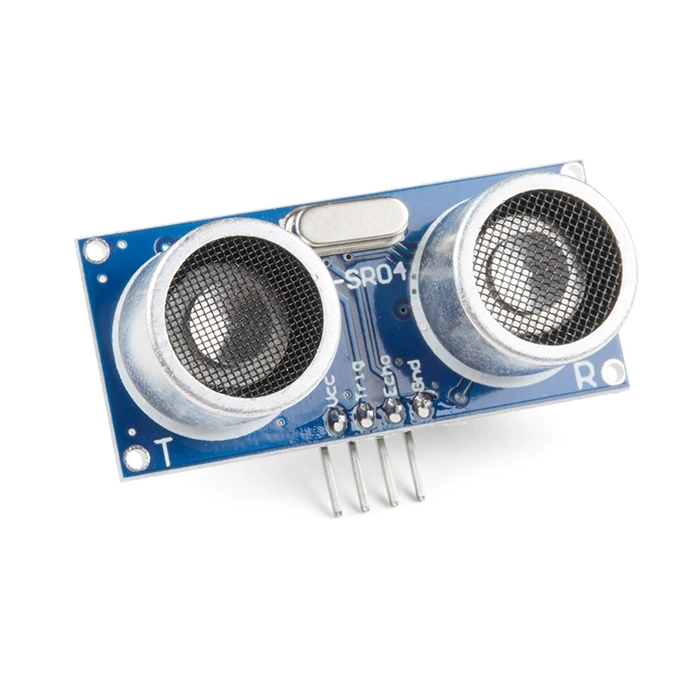
\includegraphics[width=0.5\textwidth]{img/hc-sr04.jpg}
  \\ \scriptsize
  Source: \href{https://www.sparkfun.com/ultrasonic-distance-sensor-hc-sr04.html}{SparkFun electronics}.
  \caption{HC-SR04 ultrasonic distance sensor.}
  \label{fig:hc-sr04}
\end{figure}

Consider, for example, an HC-SR04 ultrasonic distance sensor, like the one shown in Fig.~\ref{fig:hc-sr04}.
This sensor measures the distance to an object with the time it takes for a burst of ultrasound emitted by the sensor to be reflected back.
It is controlled by the Arduino using two digital pins, one that the microcontroller uses to trigger the burst to be emitted and another used by the sensor to signal that the echo has arrived.
These pins are labelled \emph{Trig} and \emph{Echo}, respectively.

Arduino rovers often have multiple ultrasonic sensors, for obstacle avoidance.
In this case, it is useful to group the pins of each sensor in a single variable to make the code more compact.
This can be accomplished with a \texttt{struct}, like shown in the program \texttt{UltrasonicStruct.ino}.

An \texttt{Ultrasonic} 

\inofile{UltrasonicStruct.ino}
\section{Classes and Objects}


%%% Local Variables:
%%% TeX-master: "main"
%%% eval: (adaptive-wrap-prefix-mode t)
%%% eval: (visual-line-mode t)
%%% eval: (nlinum-mode t)
%%% TeX-engine: luatex
%%% End:

\chapter{Libraries: Standing on the Shoulders of Giants}
\emph{Nani gigantum humeris insidentes}

\chapter{Embedded Systems Functionality}
\section{Digital Input and Output}
\section{Analog Input and Output}
\section{Pulse-Width Modulation}
\section{Servomotor control}

\printbibliography 

\end{document}

%%% Local Variables:
%%% eval: (adaptive-wrap-prefix-mode t)
%%% eval: (visual-line-mode t)
%%% eval: (nlinum-mode t)
%%% TeX-engine: luatex
%%% End:
